\subsubsection*{1.(1)}
図1の波形は奇関数なので
\begin{align*}
  A_n=0
\end{align*}
である.
Fourier正弦係数は
\begin{align*}
  B_n=&\frac{1}{\pi}\int_0^{2\pi}f(x)\sin nxdx\\
  =&\frac{1}{\pi}\left(\left(\int_\theta^{\frac{\pi}{2}-\theta}+\int_{\frac{\pi}{2}+\theta}^{\pi-\theta}\right)V\sin nxdx+\left(\int_{\pi+\theta}^{\frac{3\pi}{2}-\theta}+\int_{\frac{3\pi}{2}+\theta}^{2\pi-\theta}\right)(-V)\sin nxdx\right)\\
  =&\frac{2V}{\pi}\left(\int_\theta^{\frac{\pi}{2}-\theta}+\int_{\frac{\pi}{2}+\theta}^{\pi-\theta}\right)\sin nxdx\\
  =&\frac{2V}{n\pi}\left(\cos n\theta-\cos\left(\frac{n\pi}{2}-n\theta\right)+\cos\left(\frac{n\pi}{2}+\theta\right)-\cos(n\pi-n\theta)\right)\\
  =&\frac{4V}{(2m+1)\pi}\Bigl(\cos(2m+1)\theta+(-1)^{m+1}\sin(2m+1)\theta\Bigr)
\end{align*}
ここで$m$は非負整数である.実際に$0\leq m\leq20$でプロットすると図\ref{fig:fig/fig1.png}のようになる.
\begin{figure}[htbp]
  \begin{center}
    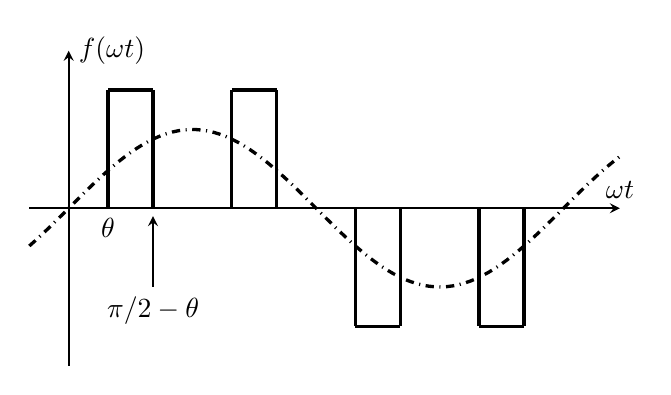
\begin{tikzpicture}
      \draw[->,>=stealth,semithick] (-0.5,0)--(7,0)node[above]{$\omega t$}; %x軸
      \draw[->,>=stealth,semithick] (0,-2)--(0,2)node[right]{$f(\omega t)$}; %y軸
      \draw[dash dot,samples=100,very thick,domain=-0.5:7] plot(\x,{sin(\x r)});
      \draw[very thick] (0.5,0)--(0.5,1.5);
      \draw[very thick] (pi/2-0.5,0)--(pi/2-0.5,1.5);
      \draw[very thick] (0.5,1.5)--(pi/2-0.5,1.5);
      \draw[very thick] (pi-0.5,0)--(pi-0.5,1.5);
      \draw[very thick] (pi/2+0.5,0)--(pi/2+0.5,1.5);
      \draw[very thick] (pi/2+0.5,1.5)--(pi-0.5,1.5);
      \draw[very thick] (pi+0.5,0)--(pi+0.5,-1.5);
      \draw[very thick] (pi*3/2-0.5,0)--(pi*3/2-0.5,-1.5);
      \draw[very thick] (pi+0.5,-1.5)--(pi*3/2-0.5,-1.5);
      \draw[very thick] (2*pi-0.5,0)--(2*pi-0.5,-1.5);
      \draw[very thick] (pi*3/2+0.5,0)--(pi*3/2+0.5,-1.5);
      \draw[very thick] (2*pi-0.5,-1.5)--(pi*3/2+0.5,-1.5);
      \draw (0.5,0) node[below]{$\theta$};
      \draw[->,>=stealth,semithick] (pi/2-0.5,-1)node[below]{$\pi/2-\theta$}--(pi/2-0.5,-0.1);
    \end{tikzpicture}
  \end{center}
  \caption{波形}
\end{figure}
\mfig[width=6cm]{fig/fig1.png}{$0\leq m\leq20$でのプロット}
\subsubsection*{1.(2)}
波形の実効値は
\begin{align*}
  V_{\rm eff}=&\sqrt{\frac{1}{2\pi}\int_0^{2\pi}(f(x))^2dx}\\
  =&\sqrt{\frac{1}{2\pi}\left(\int_\theta^{\frac{\pi}{2}-\theta}+\int_{\frac{\pi}{2}+\theta}^{\pi-\theta}+\int_{\pi+\theta}^{\frac{3\pi}{2}-\theta}+\int_{\frac{3\pi}{2}+\theta}^{2\pi-\theta}\right)V^2dx}\\
  =&\sqrt{\frac{1}{\pi}\left(\pi-4\theta\right)V^2}
\end{align*}
である.
波形のFourier級数展開は
\begin{align*}
  f(x)=&\sum_{n=1}^\infty\frac{4V}{(2n-1)\pi}\Bigl(\cos(2n-1)\theta+(-1)^{n}\sin(2n-1)\theta\Bigr)\sin(2n-1)x
\end{align*}
であるので,基本波の実効値は
\begin{align*}
  V_1=\frac{1}{\sqrt{2}}\left(\frac{4V}{\pi}\left(\cos\theta-\sin\theta\right)\right)
\end{align*}
直流成分は
\begin{align*}
  V_0=0
\end{align*}
である.
\subsubsection*{1.(3)}
歪み率は
\begin{align*}
  {\rm  THD}=\frac{\sqrt{V_{\rm eff}^2-V_1^2-V_0^2}}{V_1}=\sqrt{\frac{\pi}{8}\frac{\pi-4\theta}{(\cos\theta-\sin\theta)^2}-1}
\end{align*}
である.これは$\theta=0$のとき${\rm THD}\simeq0.483$となり,矩形波の歪み率と一致する.